\subsection*{3.1 Components used}
This project consists of both hardware and software components. The hardware components used in this project are discussed below:

\subsubsection*{3.1.1 Johnson motor}
A Johnson motor is a brushed DC motor that contains permanent magnets. It is a high-speed motor with high torque and widely used in robotic applications. In this project, Johnson motors are used for driving the wheels of the robot.

\begin{figure}[H]
    \centering
    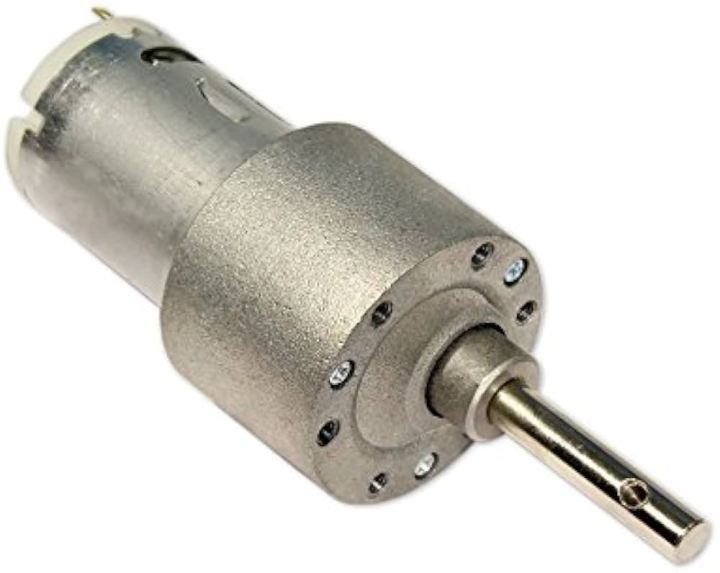
\includegraphics[width=0.5\textwidth]{3.1.jpg}
    \caption{Johnson Motor (Source: \cite{7})}
    \label{fig:3.1}
\end{figure}

\subsubsection*{3.1.2 Raspberry Pi 4}
Raspberry Pi 4 is a credit card-sized computer that can run an operating system and perform multiple functions. It is equipped with a Broadcom BCM2711, Quad core Cortex-A72 (ARM v8) 64-bit SoC @ 1.5GHz, 2GB RAM, and USB and HDMI ports. In this project, it processes voice commands, sends control signals to Arduino, and communicates with cloud services.

\begin{figure}[H]
    \centering
    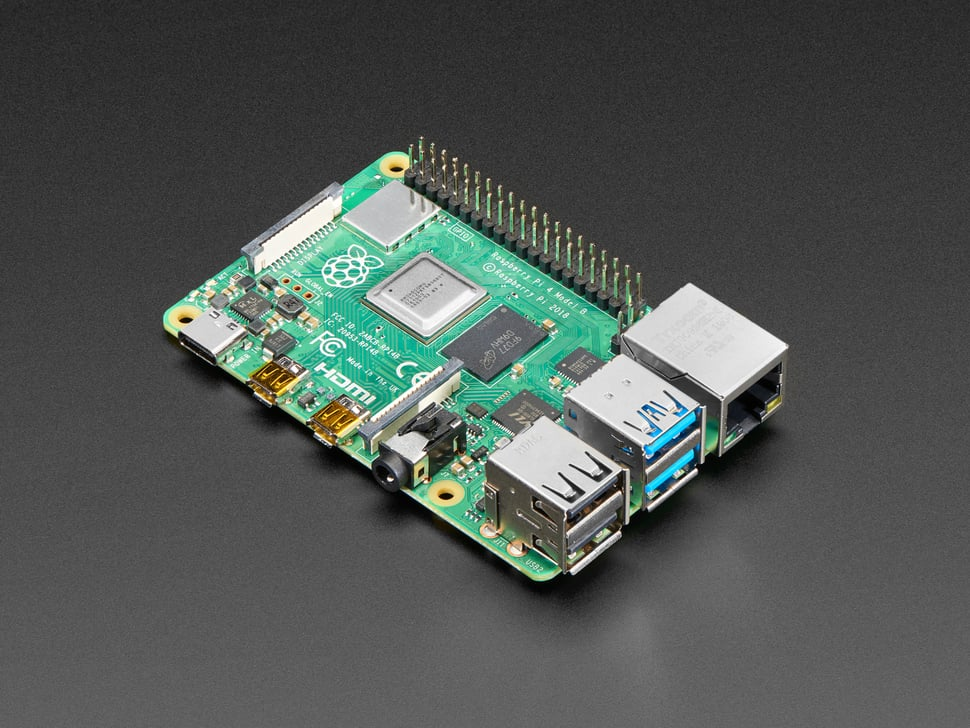
\includegraphics[width=0.5\textwidth]{fig3.2.jpg}
    \caption{Raspberry Pi 4 (Source: \cite{8})}
    \label{fig:3.2}
\end{figure}

\subsubsection*{3.1.3 Arduino UNO}
The Arduino UNO is an open-source microcontroller board based on the Microchip ATmega328P microcontroller. It features 14 digital I/O pins, 6 analog inputs, a 16 MHz quartz crystal, and USB and power jack. In this project, it controls motors and sensors based on the instructions received from the Raspberry Pi.

\begin{figure}[H]
    \centering
    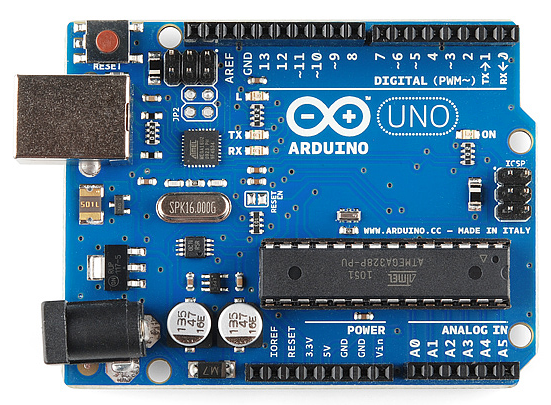
\includegraphics[width=0.5\textwidth]{fig3.3.png}
    \caption{Arduino UNO (Source: \cite{9})}
    \label{fig:3.3}
\end{figure}

\subsubsection*{3.1.4 IR Array Sensor}
IR (Infrared) array sensors are used to detect the path for line-following by emitting and detecting IR light. A group of IR sensors is arranged to detect black lines on a white surface. In this project, they help the robot follow the designated path.

\begin{figure}[H]
    \centering
    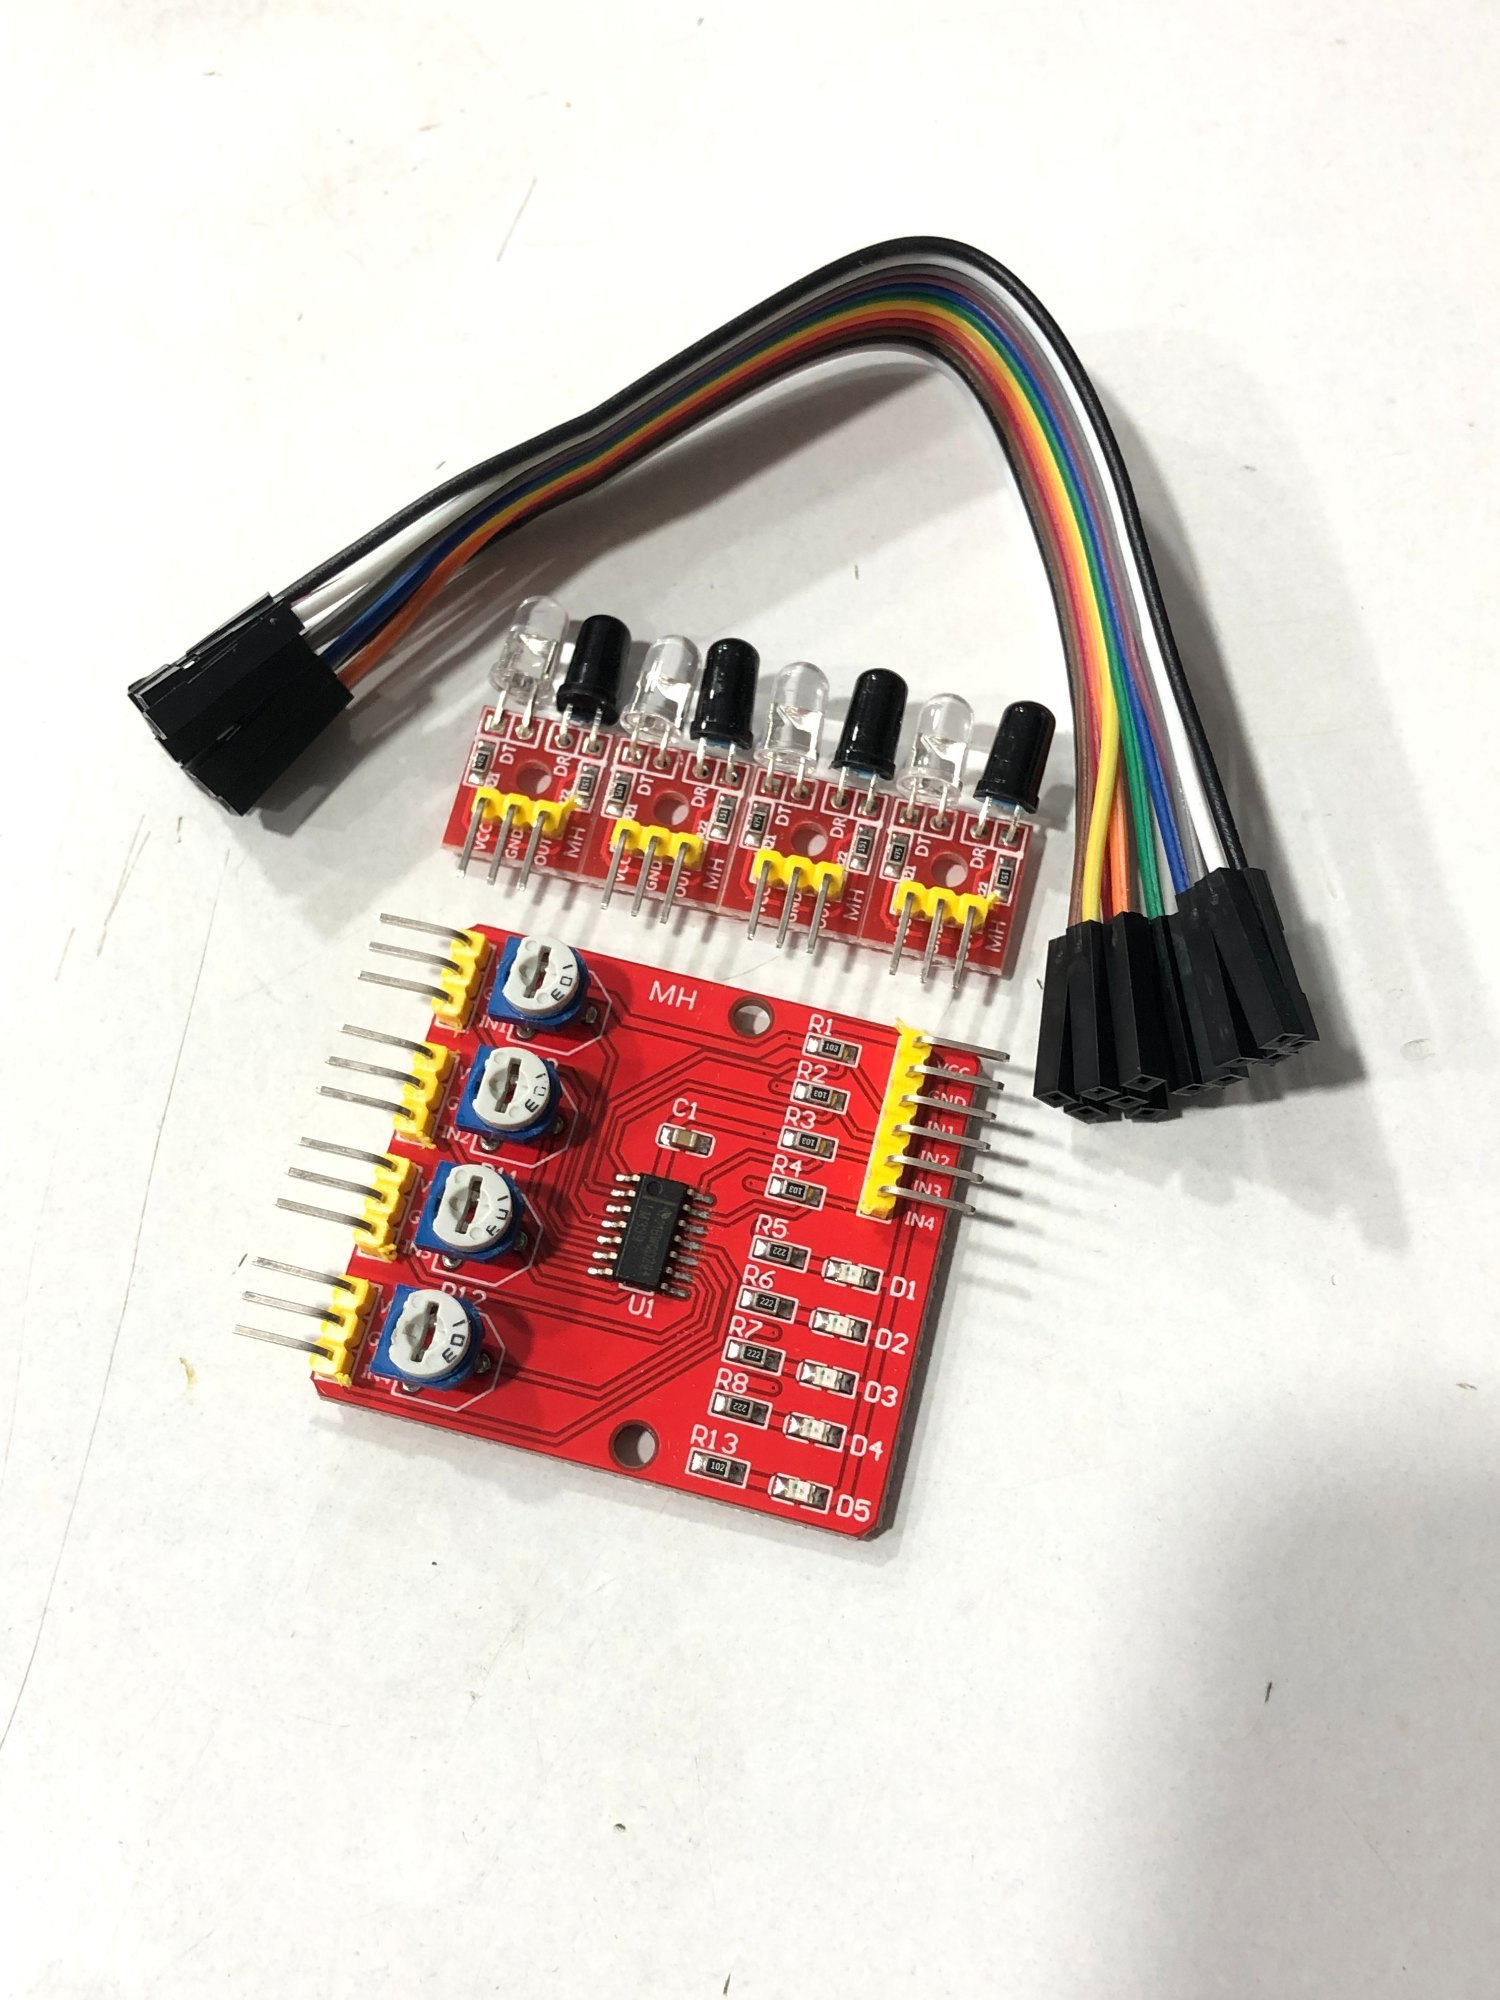
\includegraphics[width=0.5\textwidth]{3.4.jpg}
    \caption{IR Array Sensor (Source: \cite{10})}
    \label{fig:3.4}
\end{figure}

\subsubsection*{3.1.5 Metal Gear Servo MG996R}
The MG996R is a high-torque servo motor with metal gears and digital control. It provides accurate angle control and is used in the pill dispensing mechanism. It can rotate 0–180 degrees and is known for durability and stability.

\begin{figure}[H]
    \centering
    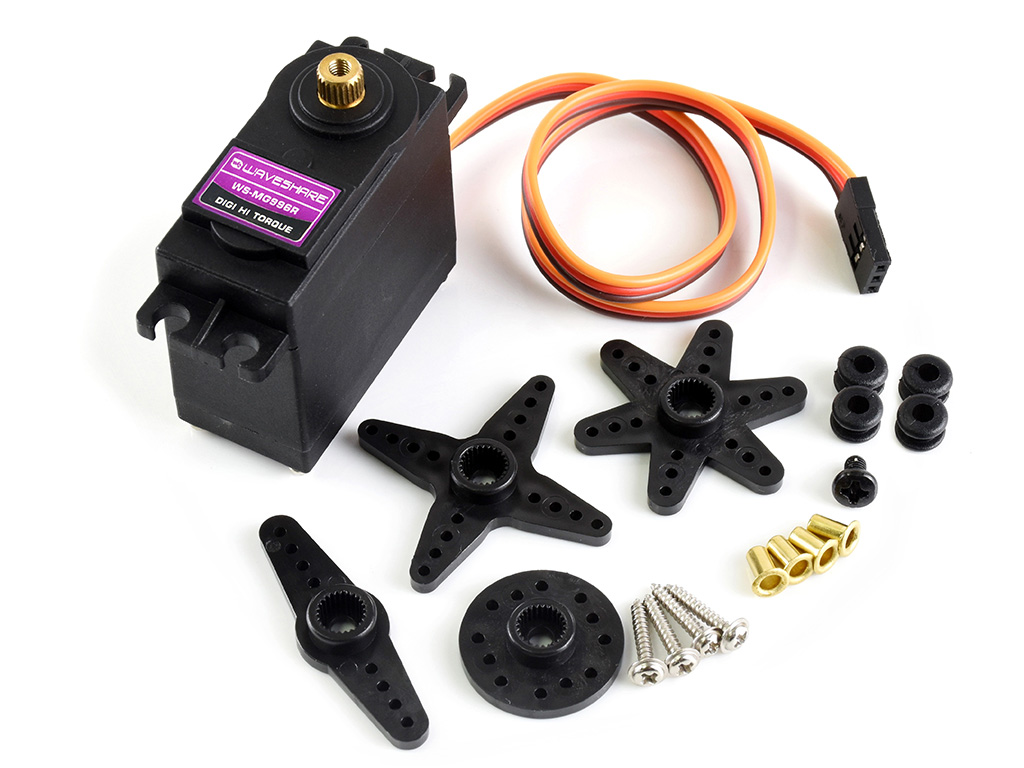
\includegraphics[width=0.5\textwidth]{3.5.jpg}
    \caption{Metal Gear Servo MG996R (Source: \cite{11})}
    \label{fig:3.5}
\end{figure}
